\documentclass[10pt,a4paper]{article}
\usepackage[italian]{babel}
\usepackage[utf8]{inputenc}
\usepackage{graphicx}
\usepackage{float}

\begin{document}

\title{Relazione Progetto\\Corso Sistemi Distribuiti}
\author{Antonio Cardace, Michele Cucchi, Federico Fossemò\\Corso Informatica Magistrale\\Università di Bologna}
\date{Aprile 2016}
\maketitle

\section{Abstract}
Il progetto implementa la realizzazione in modalità distribuita multinodo, del gioco di carte da tavolo UNO\footnote{$https://en.wikipedia.org/wiki/Uno\_(card\_game)$}. \\La relazione descrive in modo particolare i problemi affrontati, le possibili soluzioni, quelle scartate e l'implementazione definitiva.

\section{Introduzione}
L'attività di progetto ha visto la realizzazione di un'implementazione software distribuita su rete, del gioco da tavolo UNO.\\ Si è cercato di sviluppare il software focalizzandosi al massimo sull'architettura distribuita, evitando dove possibile di utilizzare paradigmi centralizzati puramente \textit{client-server}. La maggior parte del lavoro è stata concentrata sull'analisi e lo sviluppo di soluzioni per la gestione dei possibili crash e failures ai nodi del sistema, in funzione di impedire, per quanto possibile, blocchi nell'andamento del gioco. \\ La relazione è divisa in sotto sezioni: \begin{itemize}\item \textit{Aspetti progettuali}: descrive la struttura del sistema software realizzato, i problemi affrontati insieme alle soluzioni proposte e scartate\item \textit{Aspetti implementativi} descrive le scelte implementative specifiche dell'architettura realizzata, unitamente ai diagrammi delle classi ed interazioni UML\item \textit{Valutazione} confronta le soluzioni realizzate con lo stato dell'arte\item \textit{Conclusioni} commenti conclusivi e possibili miglioramenti\end{itemize}

\section{Aspetti progettuali}
\subsection{Descrizione del gioco}
UNO è un gioco di carte da tavolo che si svolge a turni. Il numero di giocatori può variare da un minimo di 2 ad un massimo di 10. Un giocatore vince una partita quando rimane senza alcuna carta in mano, quindi l'obiettivo del gioco è perdere più carte possibile nel tempo più breve possibile.\\All'inizio del gioco il mazziere assegna 7 carte a caso a ciascun giocatore, lasciando le restanti carte in un mazzo sul tavolo a dorso coperto.\\ La prima carta della pila viene lasciata visibile, perchè è la carta iniziale del gioco, la prima della pila scarti.\\ I giocatori procedono a turni, in senso orario, a partire da quello alla sinistra del mazziere, lasciando sul tavolo una carta delle proprie sette, che abbia stesso colore o stesso numero di quella lasciata scoperta. I giocatori possono spendere anche una carta speciale, ma se è colorata deve essere compatibile con il colore di quella scoperta. Non è possibile scartare più di una carta per turno. Nel caso un giocatore non avesse carte giocabili, è obbligato a pescarne una dal mazzo e se essa fosse giocabile, la dovrà spendere immediatamente, o passare il turno.\\\\ Le carte giocabili sono le seguenti:\\

\begin{itemize}
\item \textbf{19 Carte di colore Rosso} che vanno dall'1 al 9 (2 serie) più uno 0
\item \textbf{19 Carte di colore Blu} che vanno dall'1 al 9 (2 serie) più uno 0
\item \textbf{19 Carte di colore Giallo} che vanno dall'1 al 9 (2 serie) più uno 0
\item \textbf{19 Carte di colore Verde} che vanno dall'1 al 9 (2 serie) più uno 0

\item \textbf{8  Carte Stop} dei colori citati, provocano la perdita del turno di gioco al giocatore successivo, nel caso di due soli giocatori il giocatore che trova la carta può rigiocare immediatamente
\item \textbf{8  Carte Cambio Giro} dei colori citati, provocano l'inversione del senso dei turni di gioco, fino alla prossima uscita della carta
\item \textbf{8  Carte Pesca 2} dei colori citati, impongono al giocatore del turno successivo di prendere 2 carte

\item \textbf{4 Carte Pesca 4} impongono al giocatore successivo di prendere 4 carte, chi gioca la carta può scegliere il prossimo colore
\item \textbf{4 Carte Cambio Colore} giocabili in ogni momento, consente a chi l'ha giocata di decidere il colore giocabile dal giocatore successivo
\end{itemize}


\subsection{Architettura del sistema}

\subsubsection{Topologia nodi e fasi del gioco}
Il gioco sviluppato rispetta esattamente le regole descritte precedentemente, si svolge a turni e per scelta progettuale prevede la presenza di 4 giocatori, ognuno dei quali si trova in un singolo host separato.\\ L'architettura logica del software cambia la sua tipologia a seconda della fase in cui si trova il gioco.\\ Sono previste 2 fasi principali: 

\begin{enumerate}
\item\textbf{Fase di registrazione} in cui il sistema prevede una topologia \textit{client-server} dove i nodi di gioco, uno per ogni giocatore su host fisici diversi, inoltrano la richiesta di registrazione ad un nodo server centrale, che coordina e sincronizza i nodi giocatori fino all'avvio del gioco.

\item\textbf{Fase di gioco} successiva alla registrazione, in cui il server perde la sua funzione e quindi i nodi creano una rete di comunicazione tra di essi costruendo un link di tipo \textbf{token-ring peer2peer}.
\end{enumerate}
 
\subsubsection{Server}
Il modulo server ha il compito di coordinare e sincronizzare i nodi dei giocatori. Fornisce delle primitive remote di registrazione per memorizzare i giocatori che intendono partecipare al gioco, ritornando in risposta un identificativo numerico univoco. Il server inoltre, controlla che il numero dei giocatori registrati sia effettivamente 4, per verificare la possibilità di avviare il gioco. Appena viene raggiunto il numero richiesto di giocatori, parte un countdown, che fa avviare il gioco alla scadenza, anche nel caso in cui alcuni giocatori non avessero esplicitato la loro volont\'a di iniziare il gioco. \\ Il server ordina l'avvio del gioco ai nodi e quindi esaurisce la sua funzione.

\subsubsection{Nodi Peer}
I nodi peer sono i client dei giocatori, distribuiti su vari e diversi host, implementano l'ambiente grafico, la logica, gli algoritmi di fault tolerance e gestione distribuita del gioco.\\ I diversi peer eseguono una copia identica del modulo software, possono essere riconosciuti grazie all'identificativo numerico rilasciatogli dal server durante la registrazione.

\subsection{Implementazione distribuita}
L'implementazione distribuita del gioco descritto impone l'analisi e la gestione dei problemi che ne derivano, in particolare emergono alcuni problemi specifici:

\subsubsection{Registrazione ed identificazione giocatori}
Gli host dei giocatori in fase di gioco  comunicano tra loro direttamente secondo il paradigma \textbf{token ring peer2peer}, ma prima di avviare il gioco è necessaria una sincronizzazione dei giocatori presso un punto comune, anche per ragioni di identificazione reciproca. La sincronizzazione iniziale viene realizzata tramite un'implementazione temporanea, solo per l'avvio, di un sistema \textbf{client-server}. Il server è l'host comune, presso il quale i nuovi giocatori devono registrarsi, per \textit{iscriversi} al gioco.\\ L'operazione di registrazione restituisce anche un identificativo numerico univoco, che consente di riconoscere inequivocabilmente i giocatori. \\ Al termine delle operazioni di registrazione, appena sarà soddisfatta la condizione sul numero dei giocatori, verrà avviato il gioco e di conseguenza gli host si scambieranno informazioni direttamente tra loro, rendendo superflua la presenza del server.\\ Per la realizzazione sono state pensate due soluzioni:
\begin{enumerate}
\item \textbf{Server Esterno}: il server è un programma esterno, che comunica tramite un protocollo condiviso, ad esempio \textit{HTTP}, occupandosi del servizio di registrazione e terminando al verificarsi della condizione di avvio del gioco.

\item \textbf{Server Integrato}: il server è parzialmente integrato con il modulo software che esegue nei nodi di gioco, ed utilizza sempre le primitive di comunicazione usate dai nodi peer. Il processo server è uno solo e può essere in un host fisico separato dai nodi di gioco. Anche in questo tipo di soluzione, il processo server termina nel momento in cui si avvia il gioco. 
\end{enumerate}
L'implementazione definitiva realizza \underline{la seconda soluzione}, scelta per mantenere il più possibile concentrato lo sviluppo, senza disperdersi con tecnologie e linguaggi diversi, continuando  l'applicazione del paradigma di comunicazione utilizzato anche nei nodi di gioco.

\subsubsection{Gestione dei turni di gioco, su topologia token-ring}
Come è già stato detto l'andamento del gioco procede a turni si rende quindi necessario un paradigma di sincronizzazione tra i vari nodi giocatori, per stabilire inequivocabilmente chi è abilitato al gioco in ogni momento.\\ La sincronizzazione avviene grazie ad un \textit{token} trasmesso tra gli host dei giocatori in sequenza ad anello. La direzione di partenza è stabilita secondo le regole del gioco.\\ Un giocatore assume il turno quando entra in possesso del token dal nodo che ha appena giocato, al termine del turno spedisce il token al giocatore successivo. Viene quindi riprodotto l'andamento a turni del gioco reale.\\ 
La gestione dei turni risulta molto affidabile ed \textit{autogestita} dagli stessi nodi senza bisogno di entità esterne alla rete peer2peer.

\subsubsection{Gestione crash nodi e politica di fault-tolerance}
L'implementazione distribuita è vulnerabile, per la natura stessa del sistema, al crash di uno o più nodi. \\La perdita di host, infatti nel caso specifico del gioco UNO, potrebbe provocare l'impossibilità di proseguire il gioco. Nel caso di crash del nodo successivo al termine di un turno, ad esempio, l'anello si bloccherebbe, impedendo di fatto al gioco di continuare. Si avrebbe lo stesso comportamento se fosse interessato da crash l'host attualmente in possesso del token di turno.\\ La realizzazione di contromisure in grado di rendere trasparenti al resto dei nodi la perdita di uno o più host, risulta quindi obbligatoria. \\ Sono state analizzate due possibili soluzioni:

\begin{enumerate}
\item \textbf{Leader dei nodi}\\ Il leader è eletto tra i nodi con \textit{l'algoritmo del bullo}, gestisce il fault tolerance, ricevendo dai singoli host un messaggio di \textbf{alive} a cui risponde con un \textbf{ACK}, nel caso non riceva il messaggio può considerare il giocatore eliminato facendo proseguire il gioco. Se fosse crashato l'host con il token di turno, il leader ricrea e fa ripartire il token. In caso di crash dello stesso leader, il primo nodo che non riceve l'ACK reindice l'elezione per un nuovo leader. 

\item \textbf{Token di Fault-Tolerance, token di Turno e orologi vettoriali}\\ Ogni nodo memorizza lo stato dei mazzi tavolo ed un orologio vettoriale in cui registrare turno e mano di gioco. Queste strutture dati vengono aggiornate ad ogni passaggio di turno, tramite un messaggio broadcast inviato subito dopo la spedizione al nodo successivo del token di turno.\\ Nella fase di gioco avviato i nodi si passano un token di \textit{Fault Tolerance} per confermare la \textit{liveness} di ogni host. \\ Ogni nodo ha un timeout settato a: \\\begin{center}$T_{ft} = (TCPU*nNodi)+\sum_{}Dnodo$\end{center} dove \textit{TCPU} è la media del tempo di elaborazione dei singoli nodi, \textit{nNodi} è il numero dei nodi, \textit{Dnodo} è il valore medio del ritardo di comunicazione tra 2 singoli nodi.\\L'intervallo temporale descritto da questa formula è settato in un timer presente in ogni nodo che viene resettato ad ogni ricezione del \textit{Fault Tolerance Token}.\\ Nel caso di non ricezione del token, il primo timer a scadere genererà l'invio, dall'host in cui è scaduto il contatore, di un messaggio broadcast verso tutti i nodi rimasti, per lanciare la riconfigurazione dell'anello. I nodi risponderanno tutti all'host che ha generato l'evento di riconfigurazione, allegando anche il proprio orologio vettoriale, con cui ricostruire la turnazione di gioco, nel caso si fosse perso anche il token di turno. \\ In caso di crash dello stesso nodo generatore della riconfigurazione esiste un ulteriore timeout calcolato in modo da garantire l'impossibilità per due nodi diversi di rilanciare contemporaneamente la riconfigurazione dell'anello.\\ La formula di calcolo del tempo di attesa è la seguente:\begin{center}$Tattesa = T_{ft} +(T_{ft} * IdPeer)$\end{center}dove \textit{Tattesa} è il tempo di attesa calcolato e \textit{IdPeer} è l'identificativo univoco del nodo.\end{enumerate}

La soluzione scelta per l'implementazione finale è la numero 2, scelta per mantenere il più possibile i nodi paritetici e per sfruttare ancora la topologia di comunicazione token-ring. 

\section{Aspetti implementativi}
\subsection{Scelte implementative}
Si è scelto di realizzare il gioco UNO perchè è sembrato essere il più adatto e compatibile con le specifiche e vincoli progettuali, inoltre la semplicità del gioco ha consentito di concentrare lo sviluppo sugli aspetti principali, come la progettazione del sistema distribuito, invece che disperdersi sulla realizzazione di aspetti più secondari.\\
Il sistema rispetta i vincoli di specifica in modo stringente, di seguito sono analizzate le scelte e le specifiche punto per punto:

\subsubsection{Linguaggio Java e RMI}
Viene utilizzato il linguaggio Java in ogni componente del gioco in particolare per tutte le necessità di elaborazione distribuita sono sfruttate le primitive RMI mentre per l'ambiente grafico si è scelto di utilizzare il toolkit Java Swing.

\begin{figure}[H]
\begin{center}
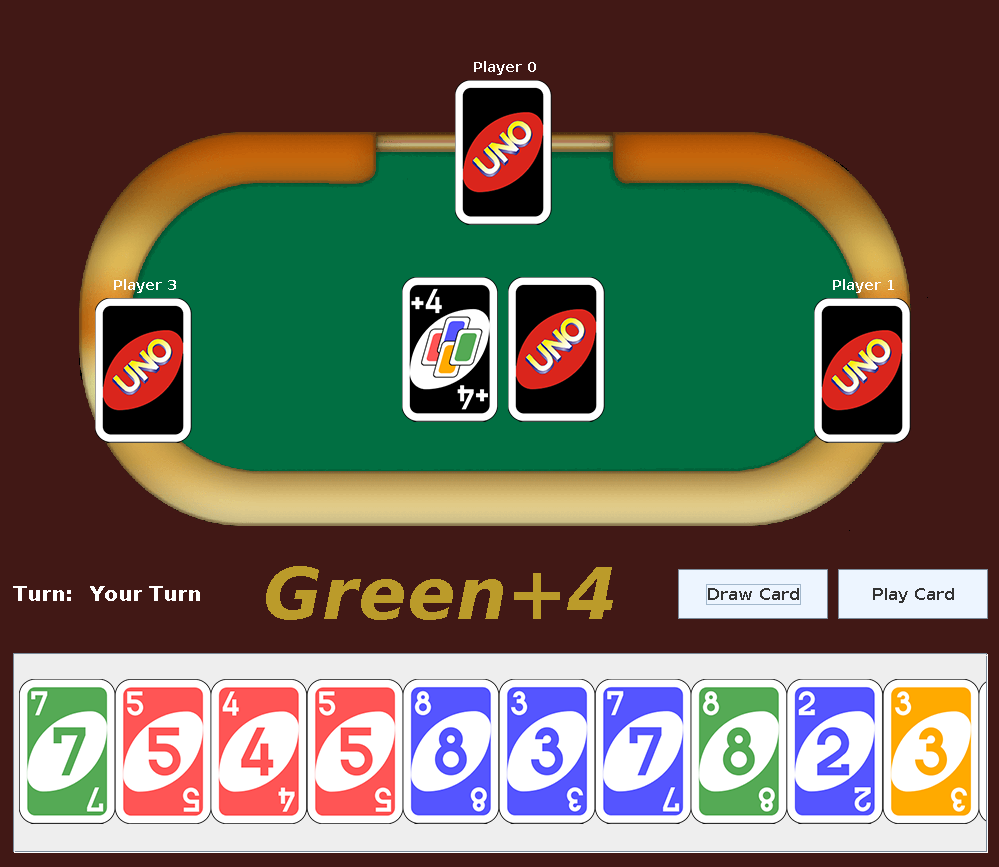
\includegraphics[height=10cm, keepaspectratio]{Selection_011.png}
\caption{Interfaccia di gioco}
\end{center}
\end{figure}

\subsubsection{Stato condiviso dai giocatori e consistenza dei dati}
Il gioco UNO prevede come stato condiviso tra i giocatori i due mazzi di carte, \textbf{nuove} e \textbf{scarti} da cui vengono prese e scartate le carte in gioco. Il comportamento è stato riprodotto mantenendo condivisi tra i nodi gli oggetti globali che rappresentano i due mazzi di carte. L'aggiornamento di questi oggetti condivisi è effettuato sulla base di messaggi broadcast inviati da ogni nodo alla fine del suo turno di gioco. L'implementazione dello stato globale condiviso consente la ricostruzione della consistenza dei dati anche in caso di crash ad uno o più host.
 
\subsubsection{Architettura distribuita, registrazione centralizzata}
L'architettura realizzata è una \textbf{token-ring} completamente distribuita, autogestita ed autoriconfigurante in caso di crash ai nodi. L'implementazione realizza l'algoritmo analizzato nel capitolo precedente. L'unica centralizzazione, nel rispetto dei vincoli di specifica, è relativa al servizio di registrazione giocatori iniziale.

\begin{figure}[H]
\begin{center}
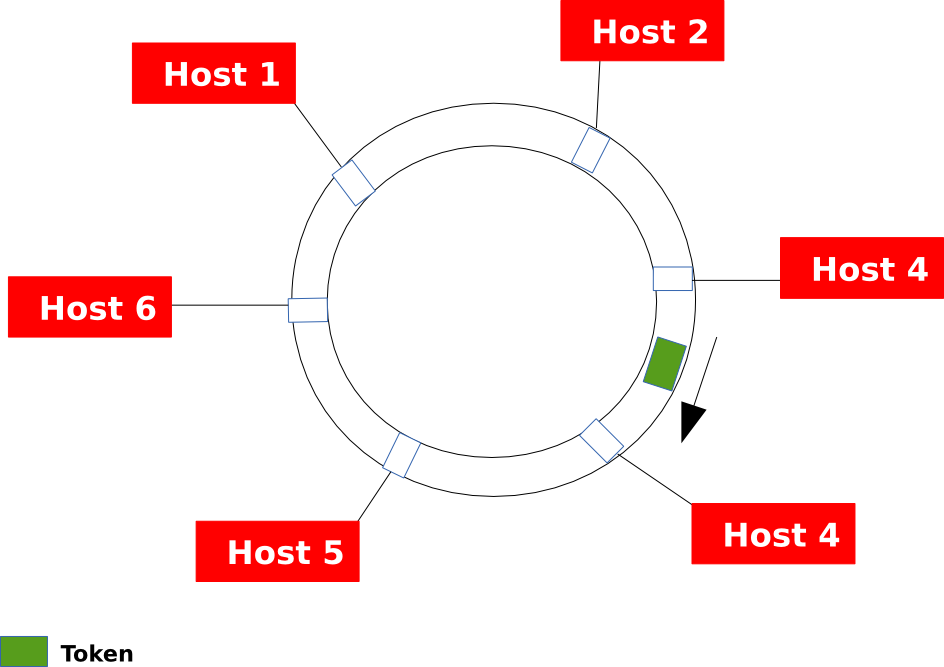
\includegraphics[height=7cm, keepaspectratio]{token-ring.png}
\caption{Esempio token-ring}
\end{center}
\end{figure}

\subsubsection{Tolleranza ai guasti}
Vengono tollerati guasti di tipo \textit{crash} ai nodi di gioco, fino alla presenza di un unico giocatore che diventa automaticamente il vincitore. La politica di recovery dai crash prevede l'inserimento delle carte appartenenti al nodo eliminato, nel mazzo scarti e la successiva eliminazione dell'host crashato dalle strutture dati comuni. I token di fault tolerance realizzano la gestione dei failure rimanendo in ambiente peer2peer, senza la necessità di host arbitri esterni.   

\subsubsection{Fault-tolerance}
Per garantire la continuità delle operazioni anche in caso di crash, le strutture dati principali, i mazzi di carte \textbf{pesca} e \textbf{scarti}, sono replicate in tutti i nodi. Al termine di un turno tutte le modifiche ai mazzi sono notificate via broadcast a tutti gli host, consentendo l'aggiornamento degli insiemi di carte, di tutti i nodi, dopo il turno giocato. Un orologio vettoriale presente in ogni nodo, incrementato ad ogni transito del token di gioco conta se il turno è stato eseguito. 


%Il sistema di fault-tolerance sviluppato implementa una topologia token-ring peer2peer, come quella realizzata per la gestione dei turni, che con  l'utilizzo di comunicazioni broadcast, strutture dati specifiche come gli \textbf{orologi vettoriali} ed il settaggio di timer per l'esecuzione delle procedure di recovery, permette la possibilità di autoriorganizzazione dei nodi senza l'utilizzo di host centralizzati. Questo tipo di implementazione ha vinto, nel confronto con la soluzione del nodo leader, anche se più complessa da realizzare, grazie alla facoltà di mantenere i nodi completamente paritetici e collaborativi tra loro, come da vincolo progettuale.



\section{Valutazione}
Lo stato dell'arte attuale prevede la tendenza all'abbandono del paradigma client-server in favore di una visione senza coordinazione centralizzata, in cui i nodi, tutti al medesimo livello fungono da \textbf{agenti} utilizzando servizi offerti da altri host o fornendo a loro volta servizi verso altri.\\ Questo tipo di topologia sta evolvendo ulteriormente verso un paradigma, chiamato \textbf{middleware} che prevede l'implementazione di certe soluzioni e l'erogazione di certi servizi, utilizzando componenti distribuite, ma emulando il comportamento di un unico host server. \\ Nell'ambito del progetto realizzato è stato utilizzato il middlware di \textbf{Distributed Object Computing} fornito dalla libreria Java \textbf{Remote Method Invocation} per costruire un sistema peer2peer puro senza coordinazione centralizzata.\\La struttura ad anello della rete dei nodi, rende semplice l'adozione di una politica principale di instradamento delle informazioni basata sul passaggio di un token tra gli host e sull'utilizzo di messaggi broadcast.\\ Durante la fase di recovery da un crash, l'instradamento delle informazioni non è più possibile tramite lo scambio di token, pertanto si attua un fallback ad una strategia di notifica attiva, basata esclusivamente sull'invio di messaggi in broadcast.\\ Soluzioni simili potrebbero prevedere lo scambio di informazioni evitando gli invii in broadcast, molto costosi per il traffico di rete, adottando invece politiche di notifica basati sul calcolo di alberi di copertura tra nodi rimasti attivi, oppure utilizzando protocolli di routing reali adattivi, probabilmente più efficienti su grosse reti. Si è scelto di utilizzare, le comunicazioni broadcast anche se intrinsecamente più costose, perchè la rete dei nodi risulta, anche nel caso peggiore, con dimensione molto limitata.\\ L'obiettivo è stato privilegiare la velocità delle notifiche rispetto all'efficienza della comunicazione. 


\section{Diagrammi}

\subsection{Interazioni}
\begin{figure}[H]
\begin{center}
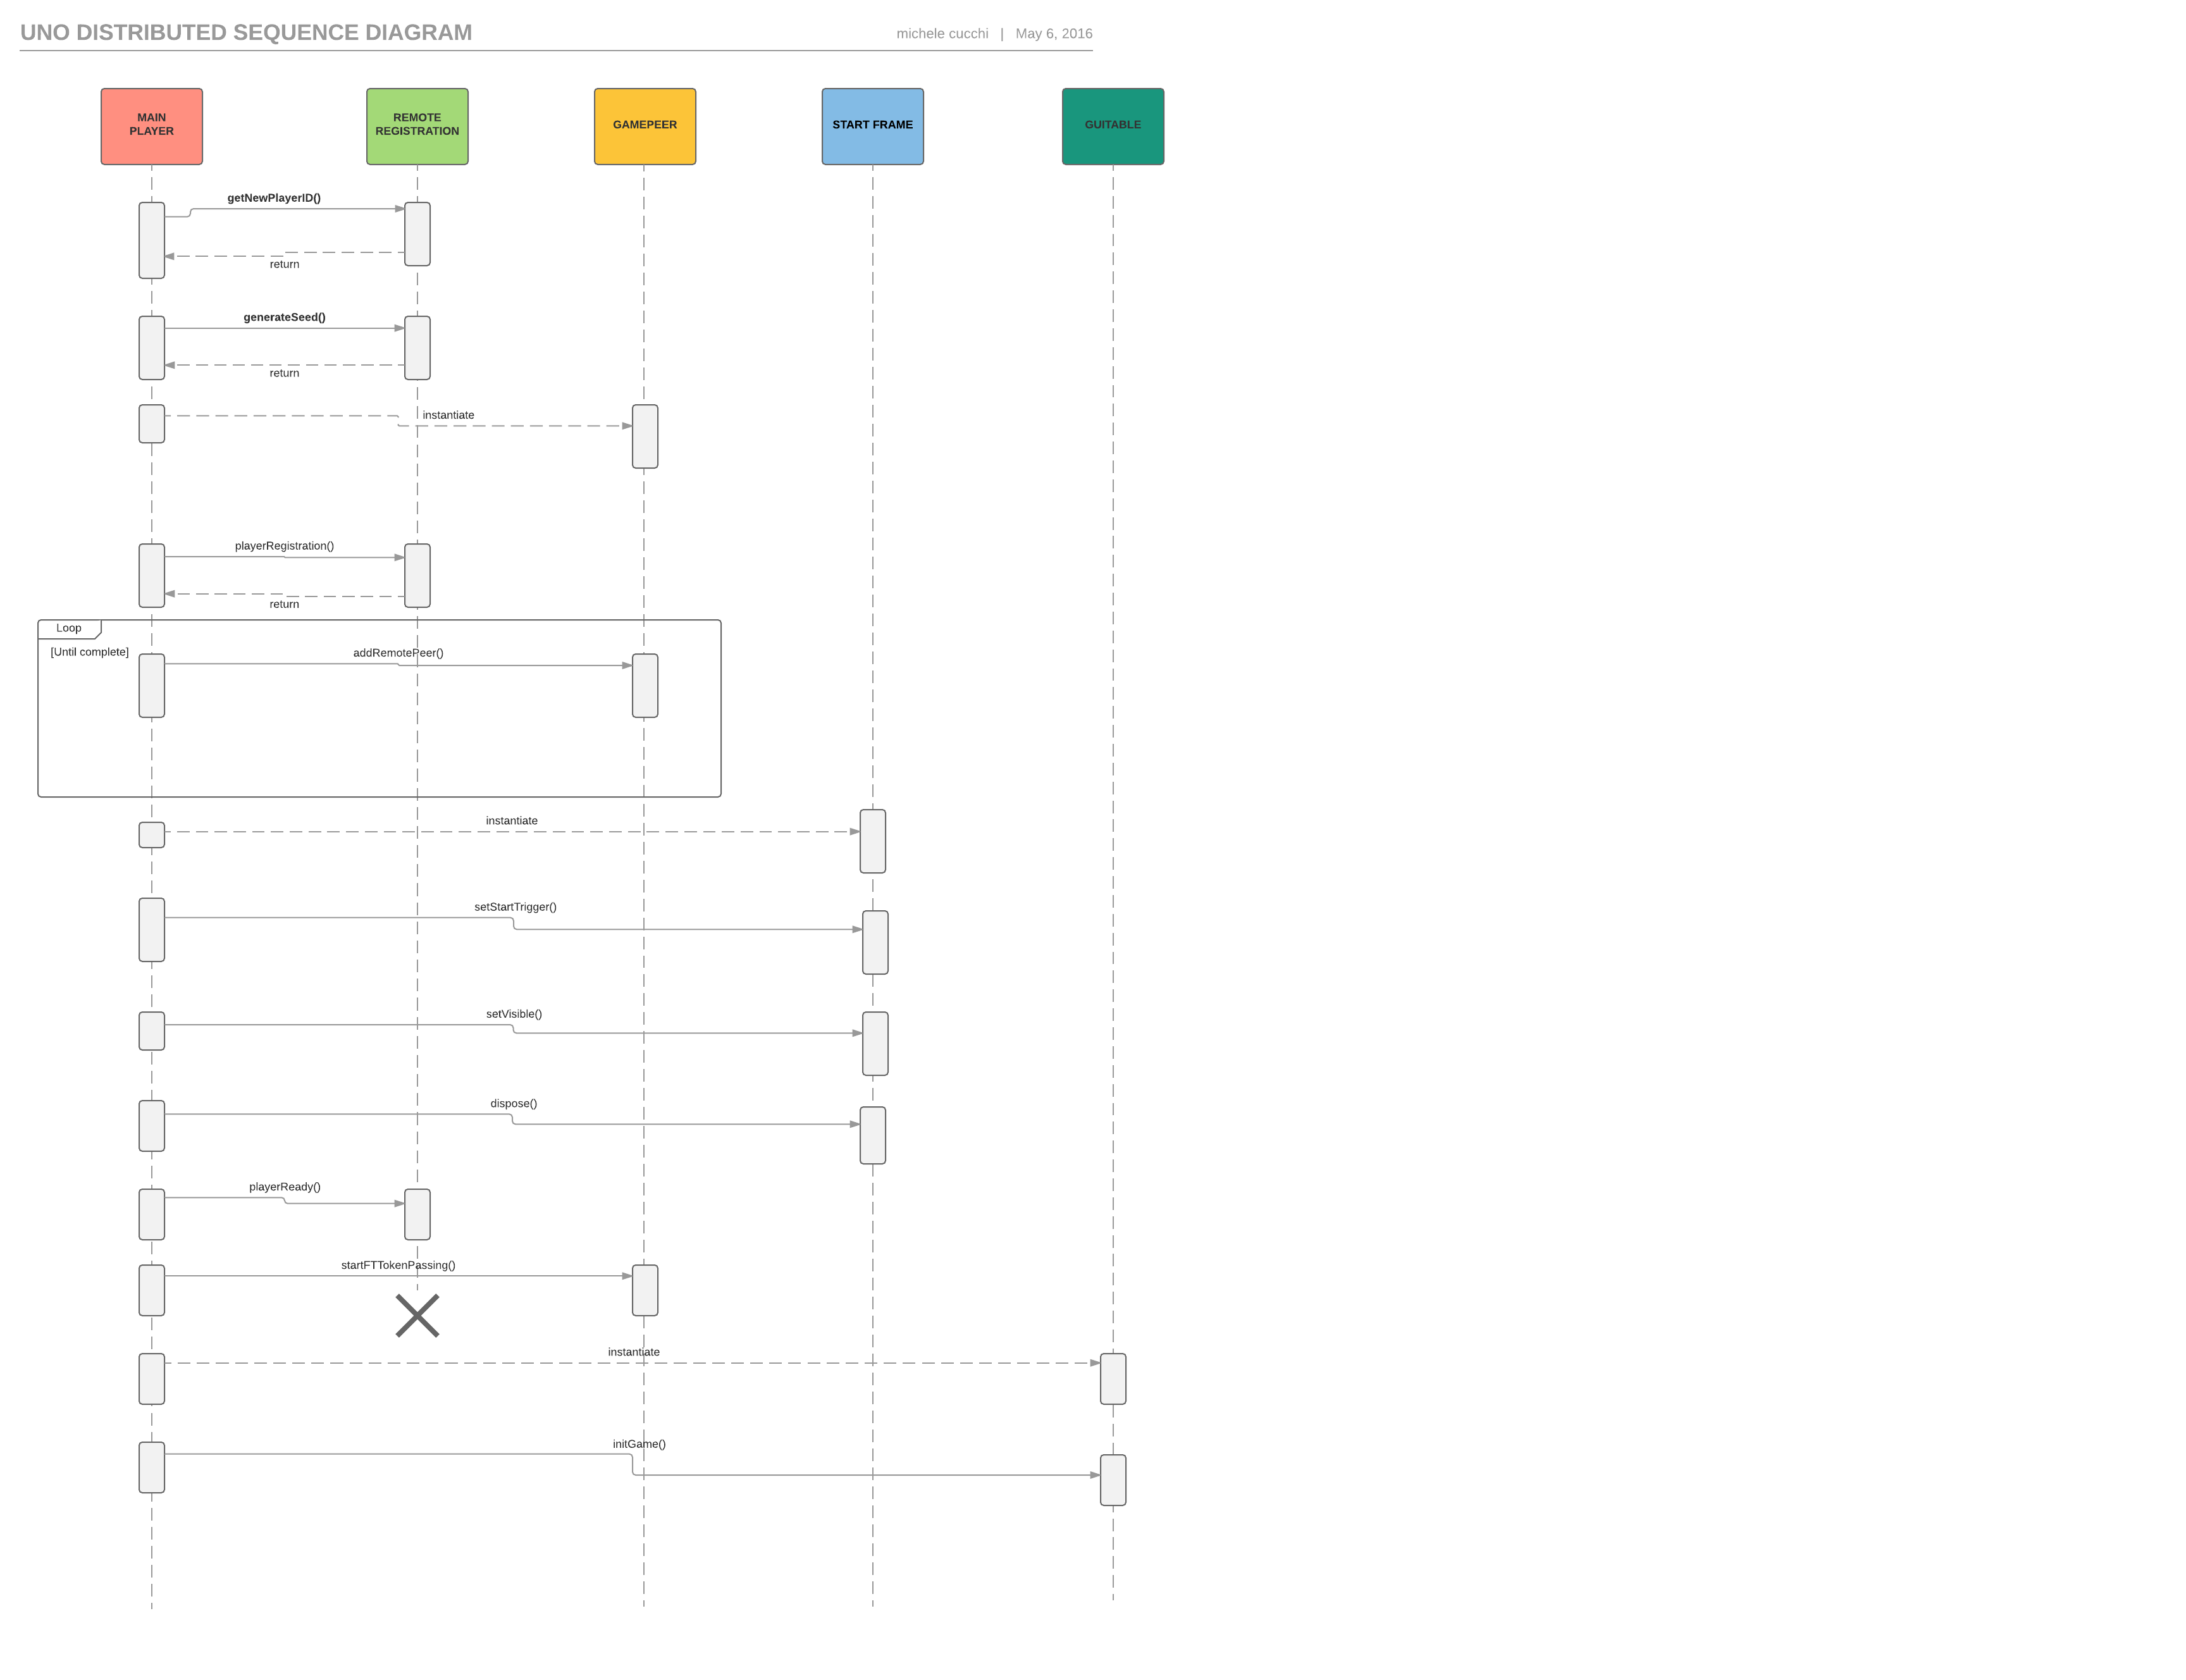
\includegraphics[height=20cm, keepaspectratio]{registration.png}
\caption{Diagramma interazioni nella fase di registrazione}
\end{center}
\end{figure}

\begin{figure}[H]
\begin{center}
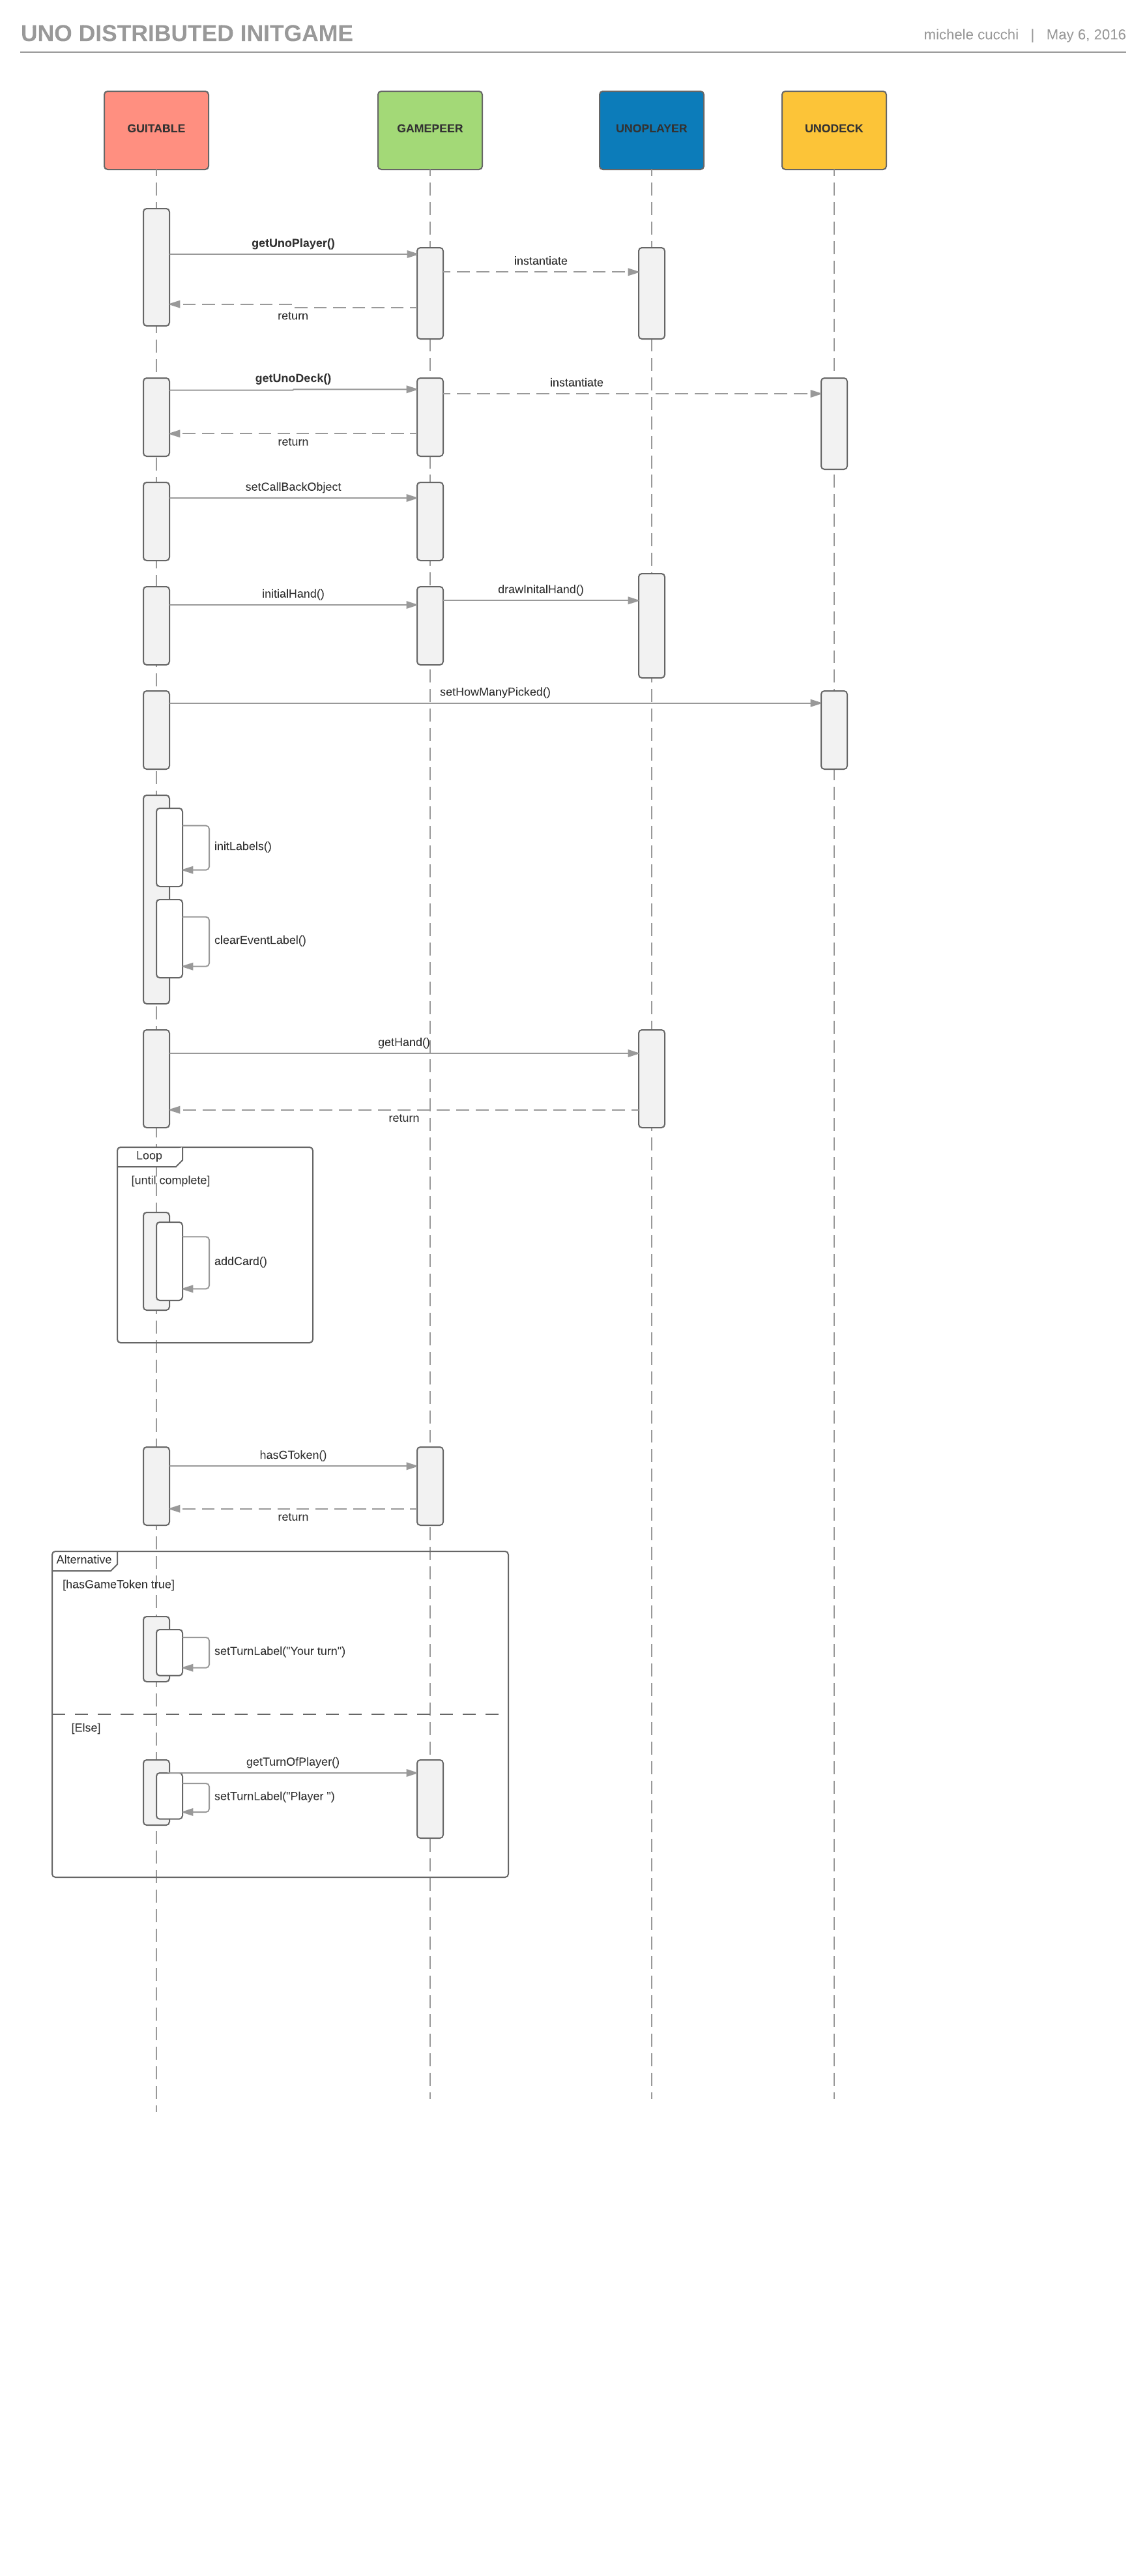
\includegraphics[height=22cm, keepaspectratio]{initgame.png}
\caption{Diagramma interazioni nella fase iniziale del gioco p2p}
\end{center}
\end{figure}

\subsection{Classi}
\begin{figure}[H]
\begin{center}
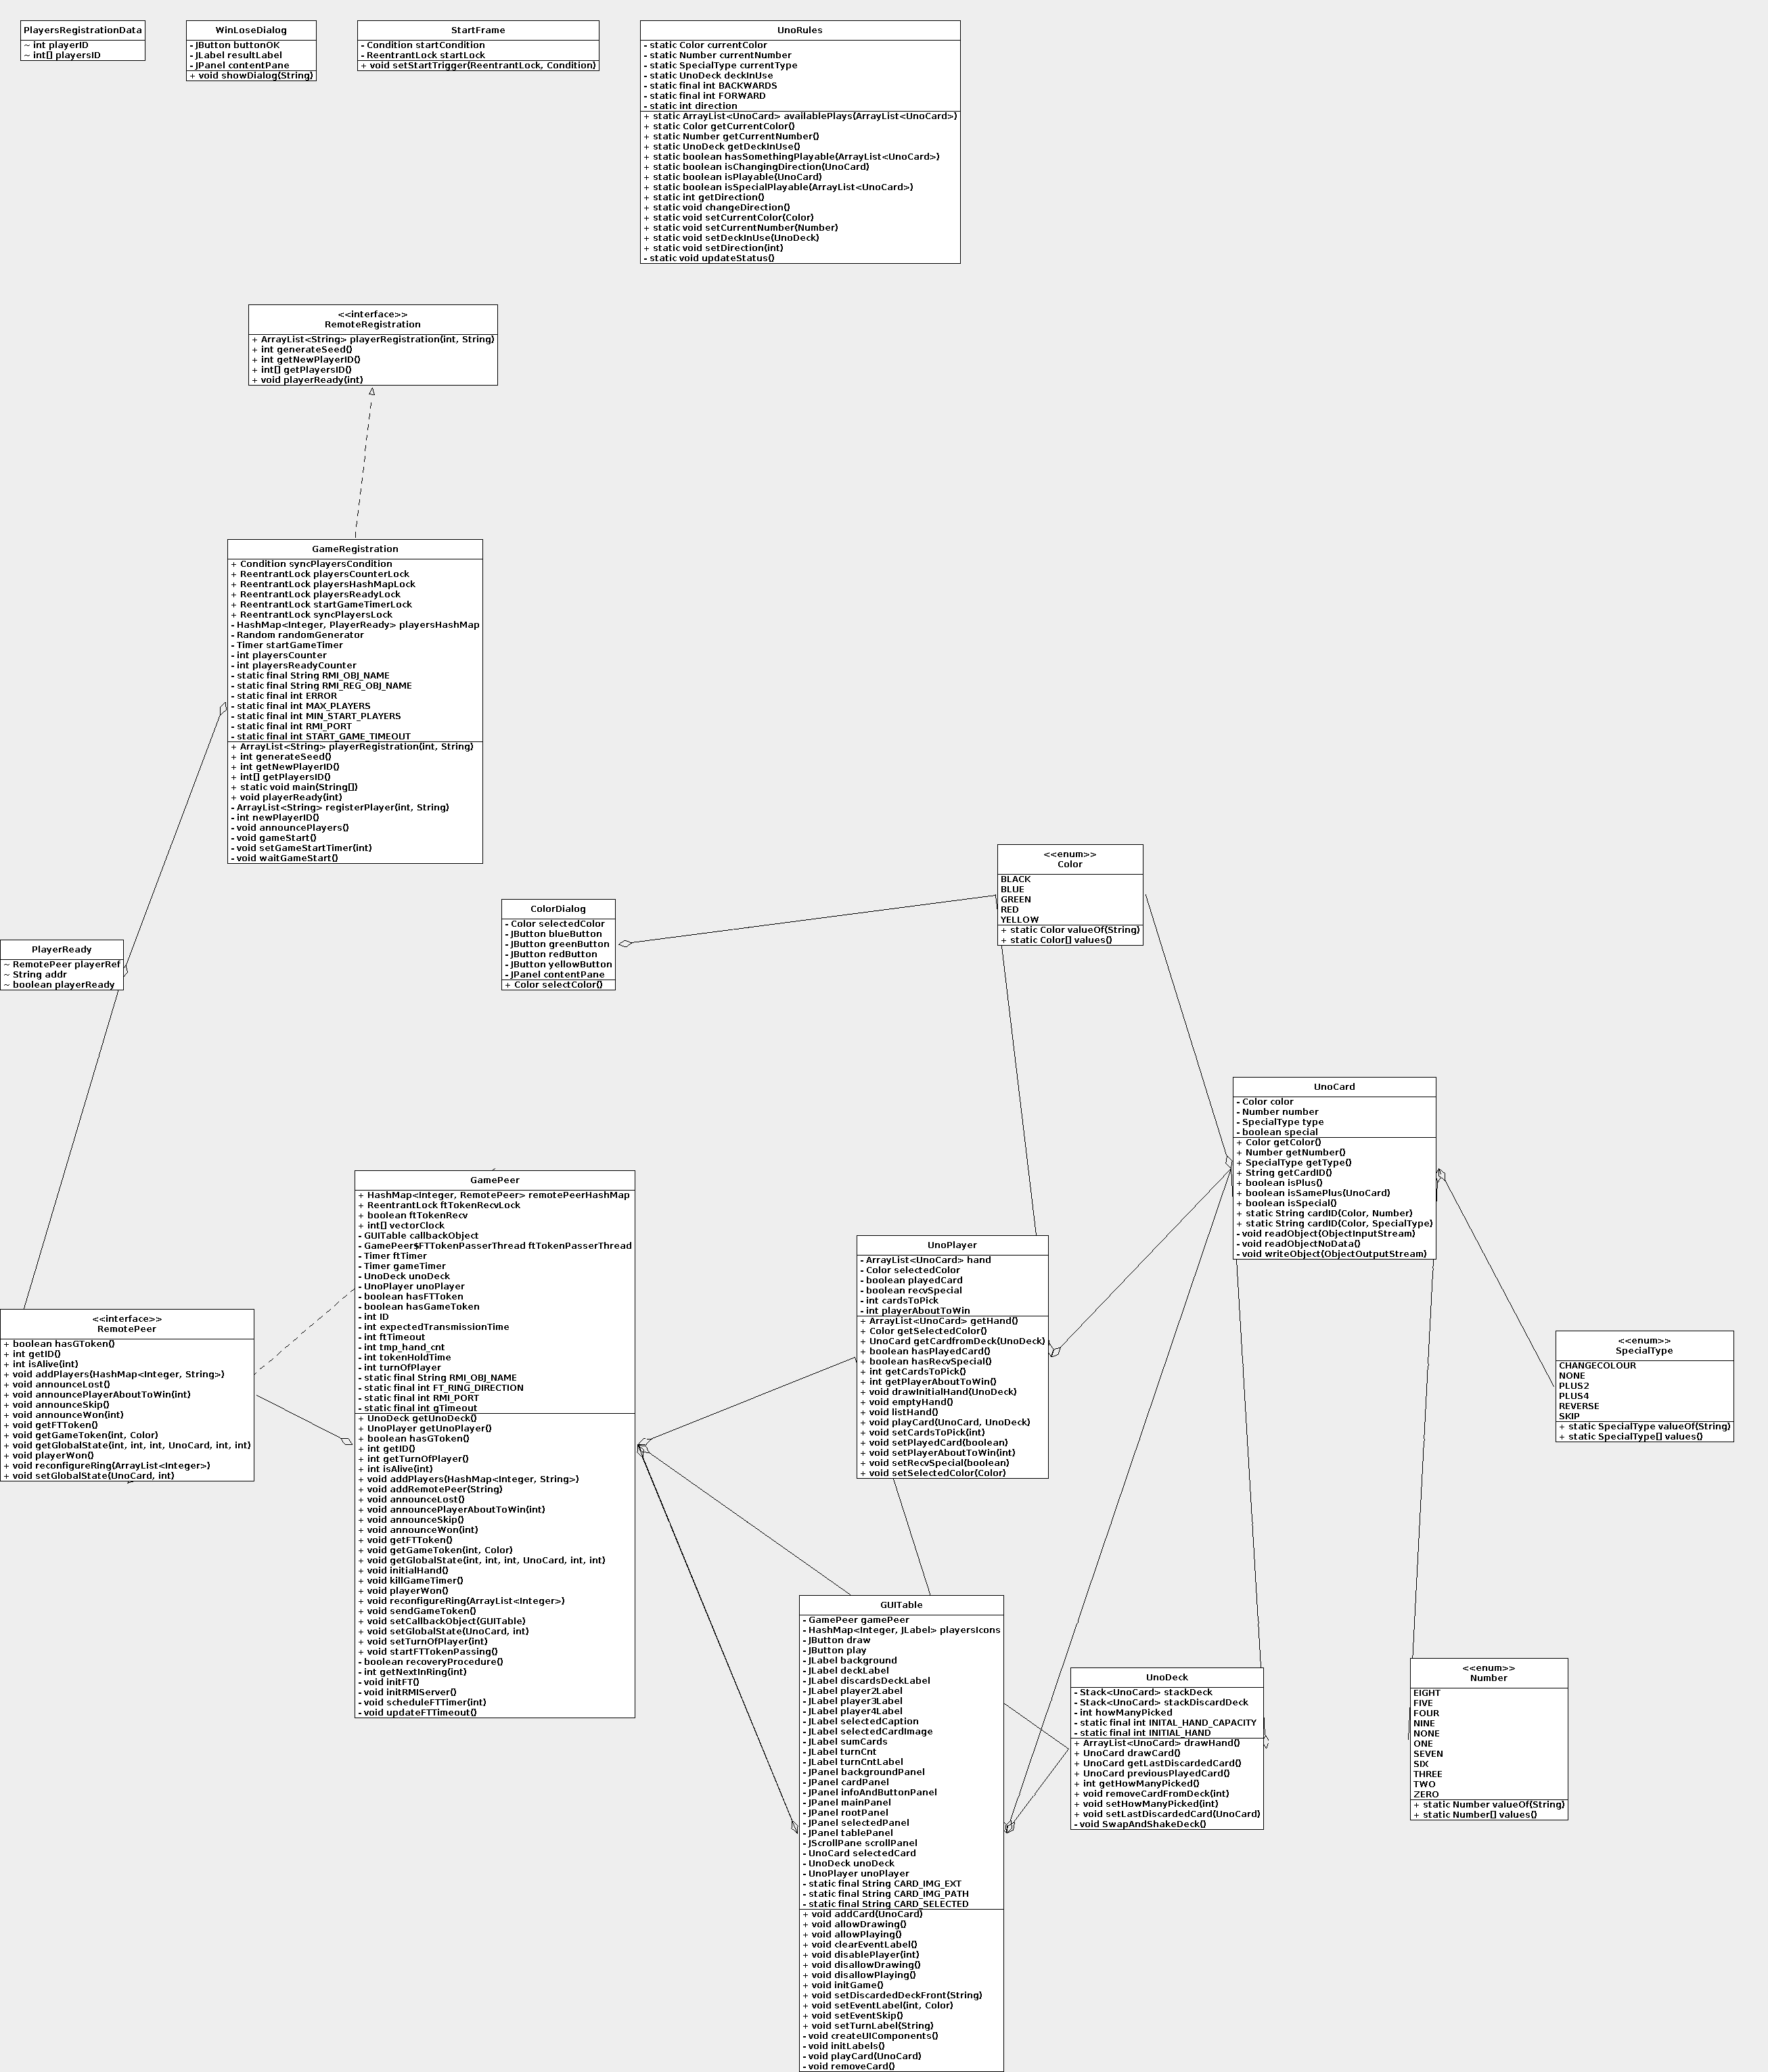
\includegraphics[width=16cm, keepaspectratio]{unogame-sd.png}
\caption{Diagramma globale delle classi}
\end{center}
\end{figure}

\section{Conclusioni}
Il lavoro di progetto ha visto l'implementazione di un gioco di carte da tavolo, utilizzando la tecnologia middleware \textbf{Distributed Object Computing} fornita dalla libreria Java \textbf{Remote Method Invocation}. L'utilizzo dei servizi Java RMI ha consentito la realizzazione di un sistema distribuito, con topologia ad anello puramente peer2peer. La politica di fault-tolerance è attuata grazie ad autogestione e riconfigurazione automatica dei nodi stessi senza interventi di agenti esterni centralizzati. \\Si può pensare ad un possibile miglioramento ed ottimizzazione futura cercando di sostituire le comunicazioni broadcast tra nodi con qualcosa di più efficiente. Inoltre potrebbe essere studiata una soluzione con sistema di registrazione anch'esso distribuito. \\ Può essere migliorata anche l'interfaccia grafica, realizzata in forma minimale e sintetica.  


\end{document}
